%cSpell:enableCompoundWords

% My mini-preamble
\newcommand{\asgn}{\gets\,}
\newenvironment{landscape}{%
\newgeometry{textwidth=\textheight,textheight=\textwidth,left=15mm,top=15mm}%
\eject\pagewidth=297mm\pageheight=210mm%
}{%
\restoregeometry%
\eject\pagewidth=210mm\pageheight=297mm%
}

% The actual content begins here.
\section{Шейкерная сортировка. Сортировка Шелла}
Все сортировки в этом и следующем вопросах сортируют массив по возрастанию.
\subsection{Шейкерная сортировка}
Шейкерная сортировка относится к так называемым сортировкам обменом и представляет
собой усложненную версию пузырьковой сортировки, которая одновременно сортирует массив
в двух направлениях, перемещая большие числа к концу массива, а маленькие --- к его началу.
В среднем и в худшем случае сортировка имеет сложность $O(n^2)$. В лучшем случае, когда
массива уже отсортирован, алгоритм имеет сложность $O(n)$.

\begin{minted}{C++}
/// Сортирует массив в порядке возрастания
/// (за что этот алгоритм?)
void ShakerSort(int *a, int count) {
  if (count <= 1) {
    return;
  }
  // Нижняя и верхняя границы неотсортированного подмассива
  int left = 0;
  int right = count - 1;
  while (left != right) {
    int last_swap = left;
    // Поднятие больших чисел к концу массива
    for (int i = left; i < right; ++i) {
      if (a[i] > a[i + 1]) {
        std::swap(a[i], a[i + 1]);
        last_swap = i + 1;
      }
    }
    right = last_swap;
    // Перемещение маленьких чисел к началу массива
    for (int i = right; i > left; --i) {
      if (a[i] < a[i - 1]) {
        std::swap(a[i], a[i - 1]);
        last_swap = i - 1;
      }
    }
    left = last_swap;
  }
}  
\end{minted}

\subsection{Сортировка Шелла}
Сортировка Шелла является усовершенствованной версией сортировки вставками. Ее идея состоит
в том, чтобы перед тем, как сортировать весь массив, упорядочить некоторые элементы,
находящиеся на определенном расстоянии друг от друга.
\begin{figure}
  \begin{center}
  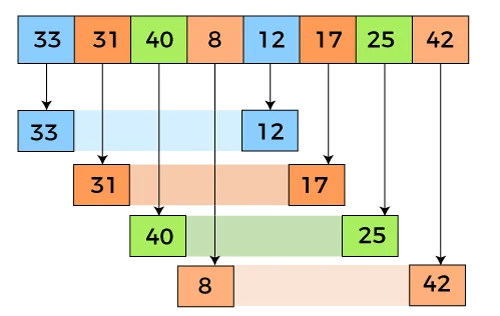
\includegraphics[scale=0.4]{27-34/shell-sort.png}
  \end{center}
  \caption{Сравнение элементов сортировкой Шелла, $h=n/2$.}
\end{figure}
Алгоритм сортирует массив в $k$ проходов. $i$-й проход характеризуется
значением смещения $h_i$, таким, что сортируются элементы, находящиеся на расстоянии
$h_i$ друг от друга. Шелл предлагал смещения $h_0 = \left\lfloor\tfrac{n}{2}\right\rfloor$,
$h_{i+1} = \left\lfloor\tfrac{h_i}{2}\right\rfloor$,
\dots, $h_{k-1} = 1$. Возможны и другие смещения, но всегда требуется, чтобы $h_{k-1} = 1$
и последовательность убывала.

На $i$-м шаге с помощью сортировки вставками между собой значения, которые можно мысленно объединить в списки вида
вида $a_{i}^{(l)}[n] = a[l+ph_i]$, где $l$ задает номер списка и индекс первого элемента
сортируемого списка в основоном массиву, а номер $p$ изменяется так в таких пределах,
чтобы элементы списка $a_{i}^{(l)}$ прошли наибольшее число элементов массива $a$,
не выходя за его пределы. Затем отсортированные списки объединяются в массив,
после чего массив вновь разбивается на списки. Данные действия повторяются ровно $k$ раз.

Сложность алгоритма сортировки Шелла зависит от выбора смещений на каждом шаге.
Ниже приведена сводная таблица некоторых схем.
\begin{longtable}{p{2cm}p{8cm}l}
  Автор   & Схема & Сложность \\ \hline
  Шелл    & см. выше & $O(n^2)$ \\
  Хиббард & \begin{minipage}{5cm} Все значения\\ $2^i - 1 \leq n\,\, \forall i \in \mathbb{N}$ \end{minipage} &  $O(n^{\frac 3 2})$ \\
  % FIXME: powers
  Седжвик & $h_i = \begin{cases}
    9\cdot 2^i - 9\cdot 2^{i/2} + 1, 2 \mid (i+1) \\
    8\cdot 2^i - 6\cdot 2^{(i+1)/2} + 1, 2 \not\mid (i+1)
  \end{cases}$ & $O(n^{\frac 7 6})$..$O(n^{\frac 4 3})$ \\
  Пратт   & \begin{minipage}{5cm} Все значения \\ $2^i \cdot 3^j \leq n/2\,\, \forall i,j \in \mathbb{N}$ \end{minipage} & $O(n\log^2 n)$ \\ \hline
\end{longtable}

\begin{minted}{C++}
/// Сортирует массив array размера size с помощью сортировки Шелла
/// использующей схему Шелла
void ShellSort(int *array, int size) {
    for (int s = size / 2; s > 0; s /= 2) {
        for (int i = s; i < size; ++i) {
            for (int j = i - s; j >= 0 && array[j] > array[j + s]; j -= s) {
                std::swap(array[j], array[j+s]);
            }
        }
    }
}
\end{minted}

\section{Сортировка Хоара – алгоритм QuickSort. Сортировка слиянием}
\subsection{QuickSort (быстрая сортировка)}
Time Complexity --- $O(n\log n)$ в среднем, $O(n^2)$
в худшем (если входной массив уже отсортирован) случае. Space Complexity зависит 
от функции разбиения (функция Хоара дает $\log n$).

Быстрая сортировка функционирует по принципу <<разделяй и властвуй>>.
Пусть требуется отсортировать массив из $n$ элементов $a[1\dots n]$ (обе границы включены).
На первом шаге полагаем $l=1$ и $r=n$. Далее придерживаемся следующего алгоритма:
\begin{enumerate}
  \item Вычислить индекс $q$ опорного элемента.
  \item Массив $a[l\dots r]$
  разбивается на два подмассива $a[l\dots q]$ и $a[q+1\dots r]$, таких что каждый элемент $a[l\dots q]$
  меньше или равен $a[q]$, который в свою очередь, не превышает любой элемент подмассива $a[q+1\dots r]$, то есть
  \begin{align*}
    \forall n <& q \quad a[n] \leq a[q] \\
    \forall m >& q \quad a[q] \leq a[m].
  \end{align*}
  \item Подмассивы $a[l\dots q]$ и $a[q+1\dots r]$ сортируются рекурсивно.
\end{enumerate}

Распространенной является функция разбиения Хоара, которая выбирает средний элемент массива
в качестве опорного.

Отметим, что в качестве опорного можно выбирать абсолютно любой элемент массива
(даже всегда первый, но при такой реализации сложность любого случая будет $\Theta(n^2)$).

Если кому-либо известен алгоритм функции разбиения, то он может злонамеренно соорудить
такой массив, на котором функция быстрой сортировки уйдет в $O(n^2)$ и/или возникнет
переполнение стека. Чтобы избежать этого, в качестве опорного можно выбирать случайный
элемент массива.

Ниже приведен алгоритм Quicksort с разбиением Хоара.
\begin{minted}{C++}
#include <iostream>
#include <utility>

/// a - массив, который сортируется
/// l - левая граница сортируемого отрезка
/// r - правая граница
int Partition(int *a, int l, int r) {
  int v = a[(l + r) / 2];
  int i = l;
  int j = r;
  while (i <= j) {
    while (a[i] < v) {
      ++i;
    }
    while (a[j] > v) {
      --j;
    }
    if (i >= j) {
      break;
    }
    std::swap(a[i++], a[j--]);
  }
  return j;
}

void Quicksort(int *a, int l, int r) {
  if (l < r) {
    int q = Partition(a, l, r);
    Quicksort(a, l, q);
    Quicksort(a, q + 1, r);
  }
}

int main() {
  int a[7] = {5, 10, -2, -3, 0, 1, 7};
  Quicksort(a, 0, 6);
  for (int i = 0; i < 7; ++i) {
    std::cout << a[i] << ' ';
  }
  std::cout << '\n';
}
\end{minted}

\subsection{Сортировка слиянием}
Данный алгоритм также использует стратегию <<разделяй и властвуй>>, рекурсивно сортируя
поданный на вход массив следующим образом:
\begin{enumerate}
  \item Массив разделяется на два подмассива так, чтобы их длины отличались не больше,
        чем на единицу;
  \item Каждый из подмассивов сортируется по отдельности рекурсивным вызовом;
  \item Посортированные массивы объединяются в один. Первый элемент результирующего 
        массива равен наименьшему из элементов подмассивов и так далее.
\end{enumerate}

Нетрудно заметить, что такая реализация потребует $O(n)$ дополнительной памяти.
Существует реализация сортировки слиянием, которая не требует дополнительной памяти,
однако она имеет большую временную сложность: $O(\log^2 n)$ против $O(\log n)$.
Ниже приведена реализация обычного алгоритма сортировки слиянием. Здесь используются
два массива, которые поочередно меняются местами. В каждом из этих массивов
в данный момент времени сортируется только одна половина исходного массива.

\begin{minted}{C++}
int *MergesortImpl(int *up, int *down, int left, int right) {
  if (left == right) {
    down[left] = up[left];
    return down;
  }

  unsigned int middle = left + (right - left) / 2;

  int *l_buff = MergesortImpl(up, down, left, middle);
  int *r_buff = MergesortImpl(up, down, middle + 1, right);

  int *target = l_buff == up ? down : up;

  unsigned int l_cur = left, r_cur = middle + 1;
  for (unsigned int i = left; i <= right; i++) {
    if (l_cur <= middle && r_cur <= right) {
      if (l_buff[l_cur] < r_buff[r_cur]) {
        target[i] = l_buff[l_cur];
        l_cur++;
      } else {
        target[i] = r_buff[r_cur];
        r_cur++;
      }
    } else if (l_cur <= middle) {
      target[i] = l_buff[l_cur];
      l_cur++;
    } else {
      target[i] = r_buff[r_cur];
      r_cur++;
    }
  }
  return target;
}

void Mergesort(int *array, int len) {
  int *back = new int[len];
  std::copy(array, array + len, back);
  int *sorted = MergesortImpl(array, back, 0, len - 1);
  if (sorted != array) {
    std::copy(back, back + len, array);
  }
  delete[] back;
}
\end{minted}

\section{Бинарные деревья – основные понятия. Основные операции с бинарными деревьями}
\subsection{Определения}
\textbf{Дерево} --- связный ациклический иерархически построенный граф. Граф обычно
полагается ориентированным в направлении иерархии: в каждую вершину (кроме одной,
называемой \textbf{корнем}) входит ровно одно ребро, но исходить из вершины может
произвольное количество ребер. Каждой вершине при этом сопоставляются какие-либо данные.

\textbf{Бинарным (двоичным) деревом} называется такое дерево, из каждой вершины которого
исходит не более двух ребер.

Когда речь идет о структурах данных, вершины принято называть \textbf{узлами}.
Данные, находящиеся в конкретном узле называют его \textbf{ключом}, а если дерево задает
отображение, то к ключам также добавляется \textbf{значения}.
% Картинка

\textbf{Ветвь} дерева --- дуга, соединяющая два узла. 

\textbf{Лист (терминальный узел)} --- узел, не имеющий исходящих ветвей.

\textbf{Внутренний узел} --- узел, имеющий как входящие, так и исходящие ветви.

Каждая ветвь задает пару \textbf{родителя} --- узла, из которого данная ветвь исходит
и \textbf{потомка} --- узла, в который данная ветвь входит. Потомками также называют
потомков потомков.

\textbf{Поддеревом} дерева называется некоторый узел вместе со всеми своими потомками.

\textbf{Глубина (уровень)} узла --- расстояние от узла до корня.

\textbf{Высота} узла --- максимальное расстояние от узла до корня. Высота дерева считается
равной высоте его корня.

% Полнота, завершенность, идеальность?
К основным операциям на деревьях относятся добавление, удаление и поиск узла (см. вопрос \ref{sec:tree-node-ops}), а также обход дерева.

\subsection{Обход}
\textbf{Обход дерева} --- посещение всех узлов дерева в определенном порядке и обработка содержащихся в них данных.
Выделяют четыре основных порядка обхода: в ширину, в прямом порядке, в обратном порядке и в симметричном порядке.
Алгоритм обхода в ширину использует $O(n)$ дополнительной памяти, остальные алгоритмы используют $O(\log n)$ памяти
на \textit{стек вызовов} {\color{red} TODO: ссылка на вопрос про стек вызовов}.

Предположим, что мы имеем дело с бинарным деревом поиска. Тогда обход в прямом порядке будет обрабатывать значения
в порядке их возрастания. Ниже приведен алгоритм обхода в прямом порядке на псевдокоде.
\begin{algorithmic}[1]
  \Function{InOrder}{Node n}
    \State Handle n
    \Comment{Обработать n}
    \If{n has left child}
      \State \Call{InOrder}{n.left}
      \Comment{Посетить левое поддерево}
    \EndIf

    \If{n has right child}
      \State \Call{InOrder}{n.right}
      \Comment{Посетить правое поддерево}
    \EndIf
  \EndFunction
\end{algorithmic}

Алгоритм обхода в обратном порядке:
\begin{algorithmic}[1]
  \Function{PostOrder}{Node n}
    \If {n has left child}
      \State \Call{PostOrder}{n.left}
    \EndIf
    \If{n has right child}
      \State \Call{PostOrder}{n.right}
    \EndIf
    \State Handle n
  \EndFunction
\end{algorithmic}

% TODO: симметричный обход

Алгоритм обхода дерева в ширину посещает дерево слой за слоем: сначала посещается корневой узел,
затем его дети (все вершины глубины 1), после них алгоритм посещает все вершины глубины 2 и так
далее, пока не будут исчерпаны все вершины.
\begin{algorithmic}[1]
  \Function{Bfs}{Node n}
    \State q $\gets$ empty Queue
    \State \Call{q.Push}{n}
    \While{q is not empty}
      \State m $\gets$ q.\Call{Pop}{}
      \State Handle m
      \If {n has left child}
        \State q.\Call{Push}{n.left}
      \EndIf
      \If{n has right child}
        \State q.\Call{Push}{n.right}
      \EndIf
    \EndWhile
  \EndFunction
\end{algorithmic}

\section{Понятие рекурсивного типа данных}
\textbf{Рекурсивным типом данных} является всякий тип данных, который в своем объявлении содержит ссылается
на себя.

С помощью рекурсивных типов реализуются узлы таких структур данных, как списки и деревья, которые
содержат ссылки на потомков и предков.

В языке \verb|C++| структура (класс, объединение) не является полным типом до конца
своего объявления, потому не может содержать саму себя в качестве поля. Действительно, если бы структура
могла содержать саму себя, то она бы имела бесконечный размер, который невозможно поместить в конечную память.

При этом структура принципиально может содержать указатель или ссылку на себя. Если структура содержит ссылку на себя
в качестве поля, то эта ссылка должна быть проинициализирована при создании объекта структуры. Объект структуры со
ссылкой на себя не может быть впервые создан с помощью какого-либо конструктора, и потому без черной магии его
создать невозможно.

Структуру, содержащую указатель на себя, возможно создать не прибегая к каким-либо ухищрениям,
и потому мы будем рассматривать только их.

\begin{minted}{C++}
// Узел дерева. Содержит ссылку на родителя и двух потомков.
template<typename T>
struct TreeNode {
  T data;
  TreeNode *parent = nullptr;
  TreeNode *left = nullptr;
  TreeNode *right = nullptr;
}
template<typename T>
struct DoubleLinkedListNode {
  T data;
  DoubleLinkedListNode* prev = nullptr;
  DoubleLinkedListNode* next = nullptr;
}
template<typename T>
struct ForwardListNode {
  T data;
  ForwardListNode *next = nullptr;
}
\end{minted}

\section{Поиск и включение для деревьев. Исключение для деревьев}
\label{sec:tree-node-ops}
\section{Сбалансированные деревья. Сортировка с помощью бинарных деревьев (кучи)}

\section{Графы и возможные формы их описания. Нахождение кратчайшего пути на графе}
Графы в программировании представляют собой обобщение деревьев и подобны графам из математики.
Каждой вершине графа сопоставляется какое-либо значение, а некоторые пары вершин соединены
ребрами.

\subsection{Способы представления}
Способы задания графов в памяти компьютера в целом такие же, как и в математике,
за исключением того, что иногда матрицы заменяют списками для оптимизации
пространственной сложности.

% TODO: Arrange the figures somehow.
\begin{figure}
\begin{center}
  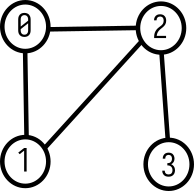
\includegraphics{27-34/sample-graph3.png}
  \caption{Граф с нумерованными (индексированными) вершинами}
  \label{fig:graph}
\end{center}
\end{figure}
\begin{figure}
\begin{center}
  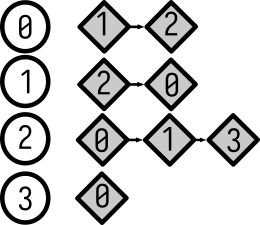
\includegraphics{27-34/adjacency-list.png}
  \caption{Список смежности}
  \label{fig:adj-list}
\end{center}
\end{figure}
\begin{figure}
  {\large $$ \begin{array}{c|c}
      & \begin{matrix} 0 & 1 & 2 & 3 \end{matrix} \\\hline
    0 & \begin{matrix} 0 & 1 & 1 & 0 \end{matrix} \\
    1 & \begin{matrix} 1 & 0 & 1 & 0 \end{matrix} \\
    2 & \begin{matrix} 1 & 1 & 0 & 1 \end{matrix} \\
    3 & \begin{matrix} 0 & 0 & 1 & 0 \end{matrix} \\
  \end{array} $$}
  \caption{Матрица смежности}
  \label{fig:adj-mat}
\end{figure}
\begin{figure}
  \begin{center}
    $$[0, 1]\rightarrow[1, 2]\rightarrow[0, 1]\rightarrow[2, 3]$$
  \end{center}
  \caption{Список ребер}
  \label{fig:edg-list}
\end{figure}


\begin{minipage}{16cm}
\begin{longtable}[]{@{}>{\raggedright}p{3cm}p{100mm}p{3cm}@{}}
  Тип представления & Описание & Занимаемое место \\ \hline
  Матрица смежности &
    Данные, соответствующие узлам графа хранятся в виде одномерного массива \verb|b|.
    Дуги графа хранятся в виде двумерного булева массива (матрицы смежности) \verb|a[i][j]|,
    причем \mverb{a[i][j] == true} тогда и только тогда, когда вершины \verb|b[i]| и \verb|b[j]|
    соединены дугой.
  & $O(E+V^2)$ \\ \hline

  Список (массив) смежности &
    Для каждой вершины хранится список (или массив) индексов смежных с ней вершин. Очень
    похоже на предыдущий пункт за исключением того, для отсутствующих ребер ничего не хранится.
  & O(V+E) \\ \hline

  Список ребер &
    Граф представляется в виде списка или массива пар индексов смежных вершин.
  & O(E) \\ \hline

  Структура с оглавлением &
    Данное представление получается из массивов смежности путем их объединения
    в один большой массив. В массиве вершин хранится индекс, с которого начинается
    ее массив смежности в объединенном массиве. Он заканчивается на индексе,
    который находится перед индексом следующей вершины.
  & O(V+E) \\ \hline
  \caption{Некоторые способы представления графов в памяти}
\end{longtable}
\end{minipage}

\subsection{Поиск кратчайшего пути}
Задача поиска кратчайшего пути отдельно рассматривается для взвешенных
и невзвешенных графов. Напомним, у взвешенных графов графов каждому
ребру поставлено в соответствие какое-либо число --- вес ребра, или длина
пути. Задача поиска кратчайшего пути на взвешенных графах сводится к поиску
такого пути от одной вершины к другой, что сумма весов ребер на этом пути минимальна.
Кратчайший путь на невзвешенных графах представляет собой такой путь, в котором
меньше всего ребер.

\subsubsection{BFS}
Для поиска пути на невзвешенных графов используется поиска в ширину. Ниже приведен псевдокод функции,
осуществляющей поиск кратчайшего пути в невзвешенном графе. Данная функция возвращает перечень вершин,
через которые надо пройти, чтобы попасть из узла $origin$ в узел $destination$, включающий эти узы.
\begin{algorithmic}
\Function{BfsPathFind}{Graph $g$, NodeIndex $origin$, NodeIndex $destination$}
\LComment{Здесь NodeIndex --- это тип индекса вершины графа.}
  \State $q$ \asgn empty Queue
  \State $visited$ \asgn empty Container
  \State $path$ \asgn empty Container
  \State $comefrom$ \asgn Array of length $g.V$
  \State $q$.\Call{Push}{$origin$}
  \While{$q$ is not empty}
    \State $n$ \asgn $q$.\Call{Pop}{}
    \State $visited$.\Call{Add}{$n$.index}
    \If{$n$ = $destination$}
      \State $visited$.\Call{Append}{$destination$}
      \While{$n \neq origin$}
        \State $n \gets visited[n]$
        \State $visited$.\Call{Append}{$n$}
      \EndWhile
      \State \Return{$path$.\Call{Reverse}{}}
    \EndIf
    \ForAll{adjacent nodes $m$ of $n$}
      \If{$m.\text{index} \notin visited$}
        \State $comefrom[m.\text{index}] \gets n$
        \State $q$.\Call{Push}{m.index}
      \EndIf
    \EndFor
  \EndWhile
  \State \Return{$path$} \Comment{Пустой путь}
\EndFunction
\end{algorithmic}
\subsubsection{A*}
Для поиска кратчайшего пути на взвешенных графах, помимо данного алгоритма, можно
использовать алгоритмы из \hyperref[sec:dijkstra_ford]{следующего вопроса.}
Прежде чем читать этот раздел, следует ознакомиться с \hyperref[sec:dijkstra]{алгоритмом Дейкстры}.

Алгоритм A* строится на основе алгоритма Дейкстры.
\section{Алгоритм Дейкстры, алгоритм Форда}
Данные алгоритмы предназначены для поиска пути на взвешенном графе.
\label{sec:dijkstra_ford}
\subsection{Алгоритм Дейкстры}
\label{sec:dijkstra}





% TODO: Place this into an appendix
% \subsection{Алгоритмы поиска}
% {\small\itshape {\bfseries \color{red} Примечание автора.\hspace{0.5em}}
% Здесь, скорее всего, подразумеваются алгоритмы обхода графа, которые также называются <<поисками>>,
% поскольку алгоритмы поиска кратчайшего пути рассматриваются в следующем вопросе.
% }

% Существует два основных алгоритма обхода графов: поиск в ширину (англ. Breadth-First Search, BFS)
% и поиск в глубину (англ. Depth-First Search, DFS).
% Их реализации практически идентичны. При одинаковом способе задания графа они также имеют
% одинаковую вычислительную сложность. Отличаются эти алгоритмы лишь порядком обхода
% графа.

% \begin{center}
% \begin{longtable}[]{@{}lc@{}}
%   Способ задания & Трудоемкость BFS и DFS \\ \hline
%   Матрица смежности & $O(V^2)$ \\
%   Список смежности & $O(V+E)$ \\
%   Матрица инцидентности & \dots \\
%   Список ребер & $O(VE)$ \\
%   Структура с оглавлением & \dots \\ \hline
% \end{longtable}
% \end{center}
  
% \subsubsection{Поиск в ширину (BFS)}
% Этот алгоритм сначала обходит соседей данной вершины графа,
% затем соседей соседей и так далее, как бы раскрывая весь граф
% слоями (сравните с одноименным алгоритмом обхода деревьев).
% Поскольку произвольный граф не имеет выраженной иерархической
% структуры, необходимо поддерживать
% \begin{algorithmic}
% \Procedure{BFS}{Graph $g$, NodeIndex origin}
% \Comment{Здесь NodeIndex --- это тип индекса вершины графа.
% Если вершины хранятся в массиве, то он будет эквивалентен какому-либо
% целочисленному типу, если нет, то это будет указатель на структуру узла.}
%   \State $q$ \asgn empty Queue
%   \State $visited$ \asgn empty Container
%   \State $q$.\Call{Push}{$origin$}
%   \While{$q$ is not empty}
%     \State $n$ \asgn $q$.\Call{Pop}{}
%     \State $visited$.\Call{Add}{$n$.index}
%     \State Handle $g$.nodes[$n$]
%     \ForAll{adjacent nodes $m$ of $n$}
%       \If{$m.\text{index} \notin visited$}
%         $q$.\Call{Push}{m.index}
%       \EndIf
%     \EndFor
%   \EndWhile
% \EndProcedure
% \end{algorithmic}

% \subsubsection{DFS}
% Реализацию DFS можно получить путем замены в алгоритме BFS очереди на стек:
% \begin{algorithmic}
% \Procedure{DFS}{Graph $g$, NodeIndex $origin$}
%   \State $q$ \asgn empty Stack
%   \State $visited$ \asgn empty Container
%   \State $q$.\Call{Push}{$origin$}
%   \While{$q$ is not empty}
%     \State $n$ \asgn $q$.\Call{Pop}{}
%     \State $visited$.\Call{Add}{$n$.index}
%     \State Handle $g$.nodes[$n$]
%     \ForAll{adjacent nodes $m$ of $n$}
%       \If{$m.\text{index} \notin visited$}
%         $q$.\Call{Push}{m.index}
%       \EndIf
%     \EndFor
%   \EndWhile
% \EndProcedure
% \end{algorithmic}

% Существует также рекурсивная реализация DFS, которая в качестве стека использует
% стек вызовов.
% \begin{algorithmic}
% \LComment{Переменная для индексов посещенных узлов. Может передаваться между рекурсивными вызовами по ссылке или быть глобальной.}
% \State $visited$ \asgn empty Container
% \Procedure{DFSRecursive}{Graph $g$, NodeIndex $n$}
%   \If{$n$.index $ \in visited$}
%     \State\Return
%   \EndIf
%   \State $visited$.\Call{Add}{$n$.index}z
%   \State Handle $g$.nodes[$n$]
%   \ForAll{adjacent nodes $m$ of $n$}
%     \State \Call{DFSRecursive}{$g$, $m$.index}
%   \EndFor
% \EndProcedure
% \end{algorithmic}